%\documentclass[10pt,twocolumn]{article}
\documentclass{acm_proc_article-sp}
%\usepackage{amsthm}
\usepackage{enumerate}
%\usepackage[dvips]{graphicx}
%\usepackage{color,times}

\newtheorem{theorem}{Theorem}
\newtheorem{lemma}{Lemma}
\newtheorem{corollary}{Corollary}

%\textwidth 6.5in \textheight 9.35in \oddsidemargin 0.0in
%\evensidemargin 0.0in \topmargin -0.55in
%\addtolength{\textwidth}{2.5mm} \addtolength{\columnsep}{2mm}

%\begin{abstract}
%\end{abstract}

%\documentclass[11pt]{article}
%\usepackage{mystyle}
%\usepackage{latexsym}
%\usepackage{amsmath}
%\usepackage{xspace}
%\usepackage{times}
%\usepackage{graphicx}
%\def\eps{\varepsilon}

%\setlength{\textwidth}{6.5in} \setlength{\evensidemargin}{0.0in}
%\setlength{\oddsidemargin}{0.0in} \setlength{\textheight}{8.5in}
%\setlength{\topmargin}{0.0in}
%\setlength{\baselineskip}{1.7\baselineskip}

%\usepackage{fullpage}

\makeatletter
\def\@copyrightspace{\relax}
\makeatother

\begin{document}
\title{The {\huge$r$}-Gather Problem in Euclidean Space}
\author{Esther M. Arkin\thanks{Department of Applied Mathematics and Statistics, Stony Brook University, Stony Brook, NY 11794. Partially supported by NSF (CCF-1526406). Email: esther.arkin@stonybrook.edu, jsbm@ams.stonybrook.edu.} \and Jie Gao\thanks{Department of Computer Science, Stony Brook University, Stony Brook, NY 11794. Email: \{jgao, jiezeng\}@cs.stonybrook.edu.} \and Matthew P. Johnson\thanks{Department of Mathematics and Computer Science, Lehman College, Bronx, NY 10468, and PhD Program in Computer Science, CUNY Graduate Center, NY 10016. Email: mpjohnson@gmail.com.} \and Joseph S. B. Mitchell$^{\ast}$ \and Jiemin Zeng$^{\dagger}$}
\maketitle

%\begin{abstract}
%
%\end{abstract}

\section{Introduction}
Given a set of $n$ points $P = \{p_1, p_2, \dots, p_n\}$ in Euclidean space and a value $r$, the aim of the $r$-gather problem is to cluster the points into groups of at least $r$ points each such that the largest diameter of the clusters is minimized. We have two definitions of the diameter of a cluster: the distance between the furthest pair of points and the diameter of the smallest enclosing circle.

One motivation of this version of clustering is from location privacy in wireless networking. With the ubiquitous use of GPS receivers on mobile devices, it is now common practice that the locations of these mobile devices are recorded and collected. This raised privacy concerns as location information is sensitive and can be used to identify the user of the devices. One common practice in the treatment of these location data is to adopt the $k$-anonymity criterion~\cite{Sweeney02}, which says that the locations are grouped into clusters, each of at least $k$ points. The cluster is used to replace individual locations such that any one user is not differentiated from $k-1$ others. Thus minimizing the diameter of the clusters can lead to location data with best accuracy while not intruding user privacy. 

%\section{Related Work}
The $r$-gather problem is shown to be NP-hard to approximate at a ratio better than 2 when $r > 6$ and the points are in a general metric by Aggarwal et al.\cite{Aggarwal06achievinganonymity}.  They also provide a 2-approximation algorithm.  The approximation algorithm first guesses the optimal diameter and greedily selects clusters with twice the diameter.  Then, a flow algorithm is constructed to assign at least $r$ points to each cluster.  This procedure is repeated until a good guess is found.  Note that this solution only selects input points as cluster centers.

Armon \cite{armon2011min} extended the result of Aggarwal et al. by proving it is NP-hard to approximate at a ratio better than 2 for the general metric case when $r > 2$.  He also specifies a generalization of the $r$-gather clustering problem named the $r$-gathering problem which also considers a set of potential cluster centers (refered to as potential facility locations in Armon's paper) and their opening costs in the final optimization function. They provide a 3-approximation to the min-max $r$-gathering problem and prove it is NP-hard to have a better approximation factor.  They also provide various approximation algorithms for the min-max $r$-gathering problem with the proximity requirement; a requirement for all points to be assigned to their nearest cluster center.

For the case where $r = 2$, both \cite{anshelevich2011terminal} and \cite{shalita2010efficient} provide polynomial time exact algorithms.  Shalita and Zwick's \cite{shalita2010efficient} algorithm runs in $O(mn)$ time, for a graph with $n$ nodes and $m$ edges.

%\cite{Guha:2000:HPN:892551, Karget:2000:BST:795666.796578,Svitkina:2008:LFL:1347082.1347208} focus on the min-sum version of a similar facility location problem.

\section{New Results}

For the application of protecting location privacy, the data points are actually in Euclidean spaces. Thus, we ask whether the hardness of approximation still holds in the Euclidean space. In the following, we assume that the input points are in the Euclidean plane.  

For the case where the diameter of a cluster is the diameter of the smallest covering disk, we show it is NP-hard to approximate better than $\sqrt{13}/2 \approx 1.802$ when $r=3$ and ${\sqrt{35}+\sqrt{3} \over 4} \approx 1.912$ when $r \geq 4$.

For the case where the diameter of a cluster is the distance between the furthest pair of points, then it is NP-hard to approximate better than $\sqrt{2+\sqrt{3}} \approx 1.931$ when $r=3$ or $4$ and $2$ when $r\geq5$.

%For the dual objective of maximizing $r$ given a fixed disk size, we can show the problem is NP-hard to approximate better than $2/3$, using instances in which the optimal $r$ value is 3. Can this be strengthened using instances whose optimal $r$ values are greater?

\section{Hardness Proof}

\begin{theorem}\label{thm:hardness1}
The $r$-gather problem for the case where the diameter of a cluster is measured by the furthest distance between two points is NP-hard to approximate better than a factor of $2$ when $r\geq5$.
\end{theorem}
\begin{proof}
Our reduction is from the NP-hard problem, planar 3SAT.  Given a formula in 3CNF composed of variables $x_i, i = 1,\dots,n$ and their complements $\overline{x_i}$, we construct an instance of $r$-gather on the plane.  Figure~\ref{fig:3satconstruction} illustrates a clause gadget of the clause $C = x_i \vee x_j \vee x_k$ and part of a variable gadget for $x_i$.  In the figure, each point represents multiple points in the same location, the number of which is noted in parenthesis.  All distances between groups of points connected by a line are distance 1 apart.  Note that all clusters shown in the figure have a diameter of 1.  If all clusters have a diameter of 1, then we can signify the parity of a variable by whether solid or dashed clusters are chosen.  Here the solid clusters signify a positive value for $x_i$ that satisfies the clause since the center point of the clause gadget is successfully assigned to a cluster.  Note that the variable gadget in Figure~\ref{fig:3satconstruction} swaps the parity of the signal sent away from the gadget.  We also include a negation gadget shown in Figure~\ref{fig:negation} that swaps the parity of the signal and can be used when connecting parts of the variable gadget together.  If an optimal solution to this $r$-gather construction can be found, the diameter of all clusters is 1.

%For the case where $r=3$ or $r = 4$, any clustering that has a cluster with diameter greater than 1 must have a cluster with diameter greater than or equal to $\sqrt{3}$.  A cluster with diameter $\sqrt{3}$ can be found in the clause gadget containing a point from each variable gadget and the center point.  There are no possible clusterings with a diameter greater than 1 or less than $\sqrt{3}$.  Therefore, it is NP-hard to approximate 3-gather and 4-gather better than a factor of $\sqrt{3}$.

The center point of the clause gadget must be assigned to a cluster that contains all $r$ points of one of the variable clusters or else a cluster of diameter 2 is forced.  WLOG, let the center point be clustered with the $r$ points of the $x_i$ gadget.  What results is the solid clusters in Figure~\ref{fig:3satconstruction} are selected above the triangle splitter and the dashed clusters are selected below the splitter.  The group of points at the top of the triangle splitter is unassigned to a cluster.  It must merge with one of the neighboring clusters which results in a cluster of diameter 2.  Therefore, it is NP-hard to approximate $r$-gather below a factor of 2 for $r\geq5$.
\end{proof}

\begin{figure}[htbp]
\begin{center}
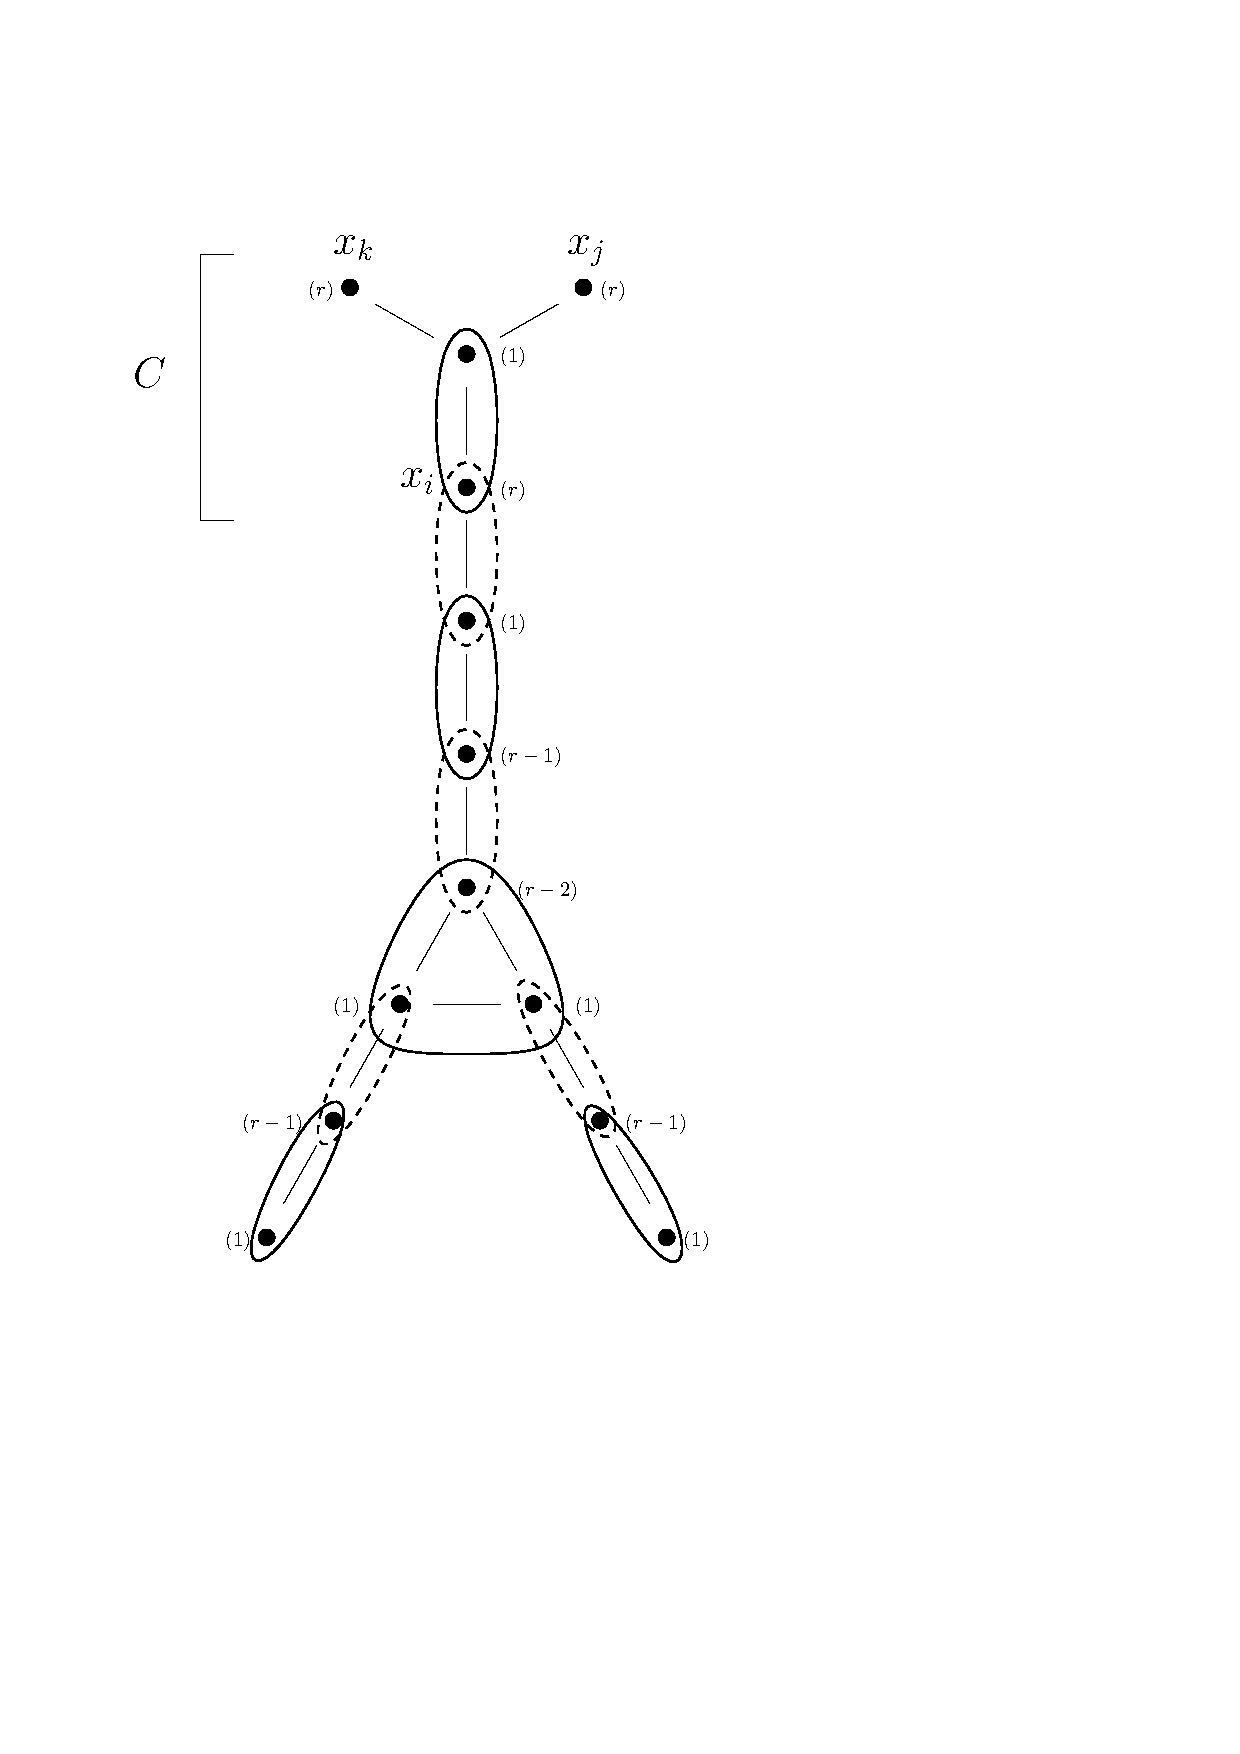
\includegraphics[scale=.6]{figs/hardness}
\caption{Clause and splitter gadget}
\label{fig:3satconstruction}
\end{center}
\vspace{-5pt}
\end{figure}

\begin{figure}[htbp]
\begin{center}
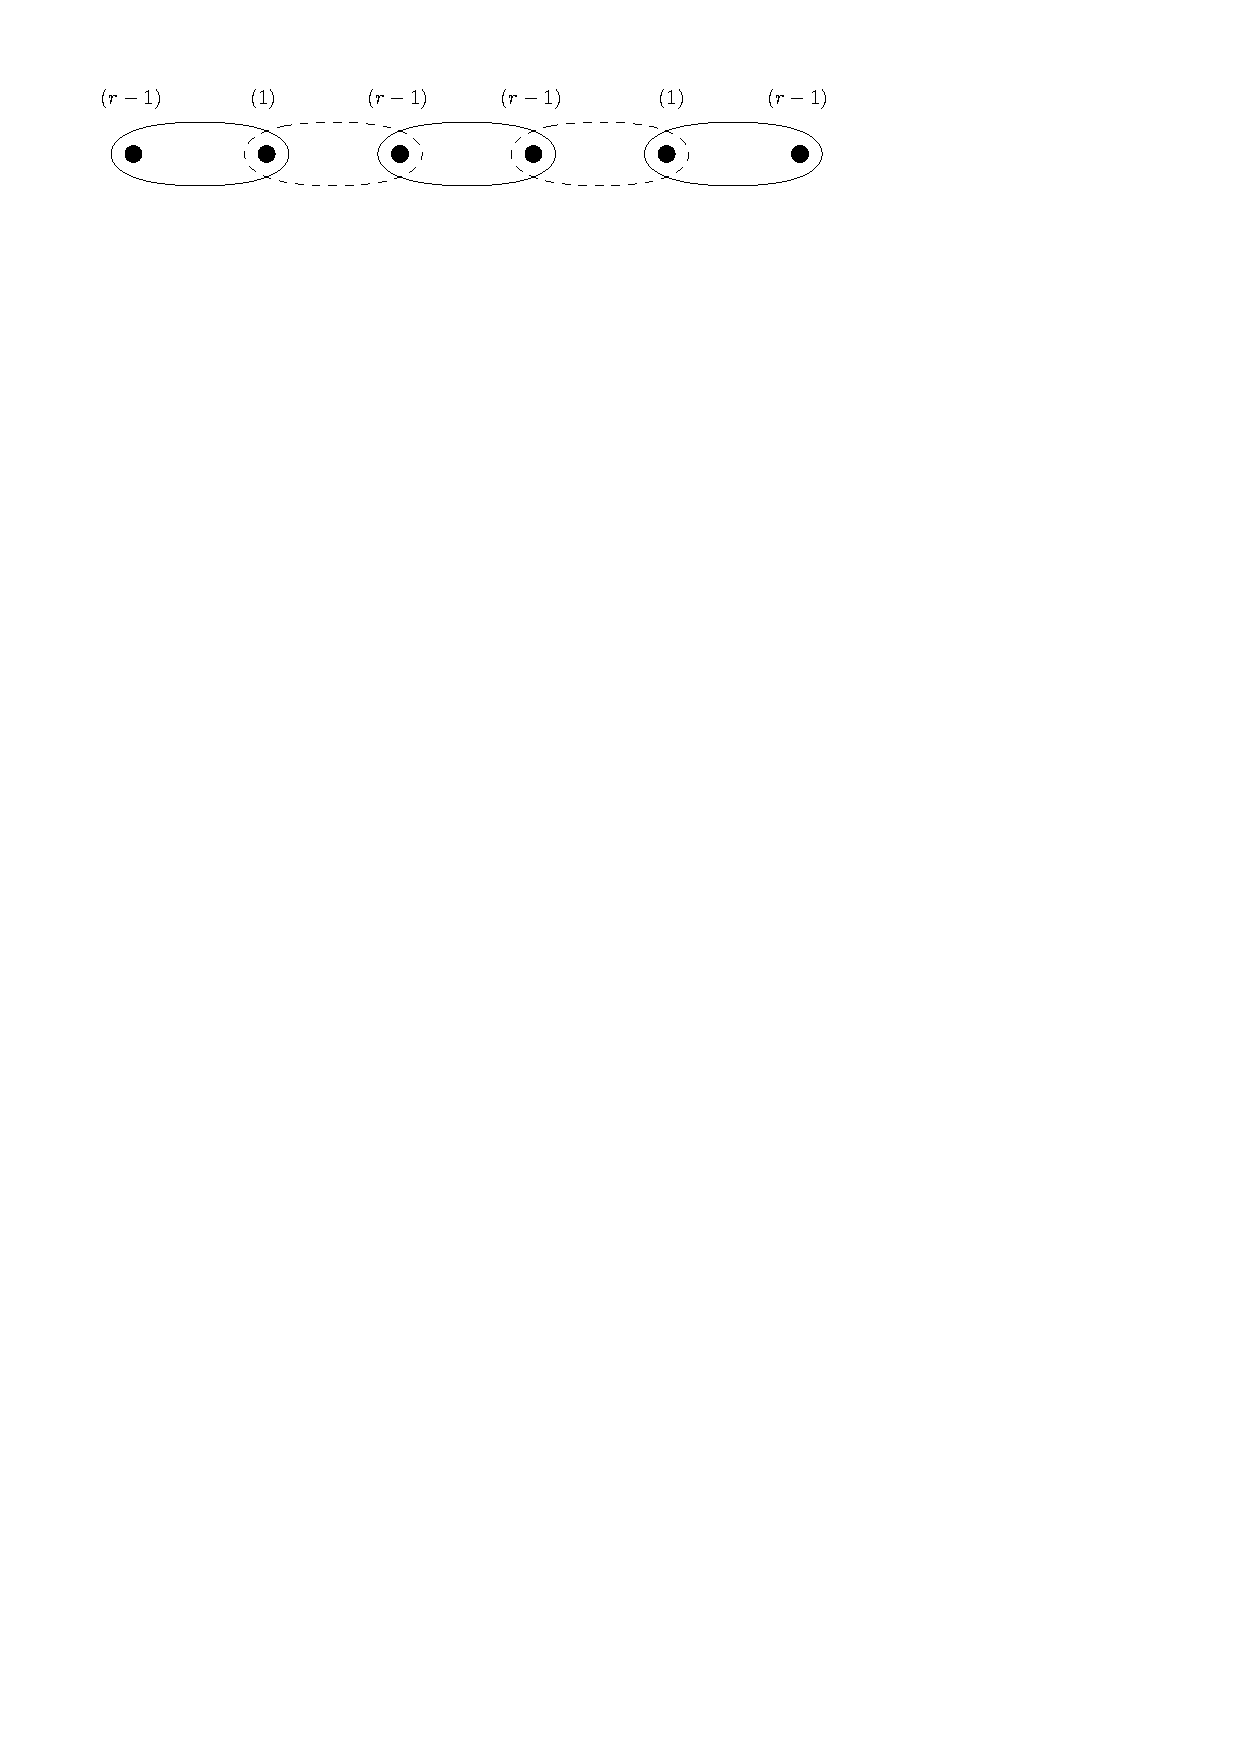
\includegraphics[scale=.6]{figs/negation}
\caption{Signal negation gadget}
\label{fig:negation}
\end{center}
\vspace{-5pt}
\end{figure}

\begin{theorem}\label{thm:hardness2}
The $r$-gather problem for the case where the diameter of a cluster is measured by the diameter of the smallest covering disk is NP-hard to approximate better than a factor of ${\sqrt{35}+\sqrt{3} \over 4} \approx 1.912$ when $r\geq4$.
\end{theorem}
\begin{proof}
The reduction is very simlar to the proof of Theorem~\ref{thm:hardness1}.  The only difference is the splitter which is illustrated in Figure~\ref{fig:splitter}.
\end{proof}

\begin{figure}[htbp]
\begin{center}
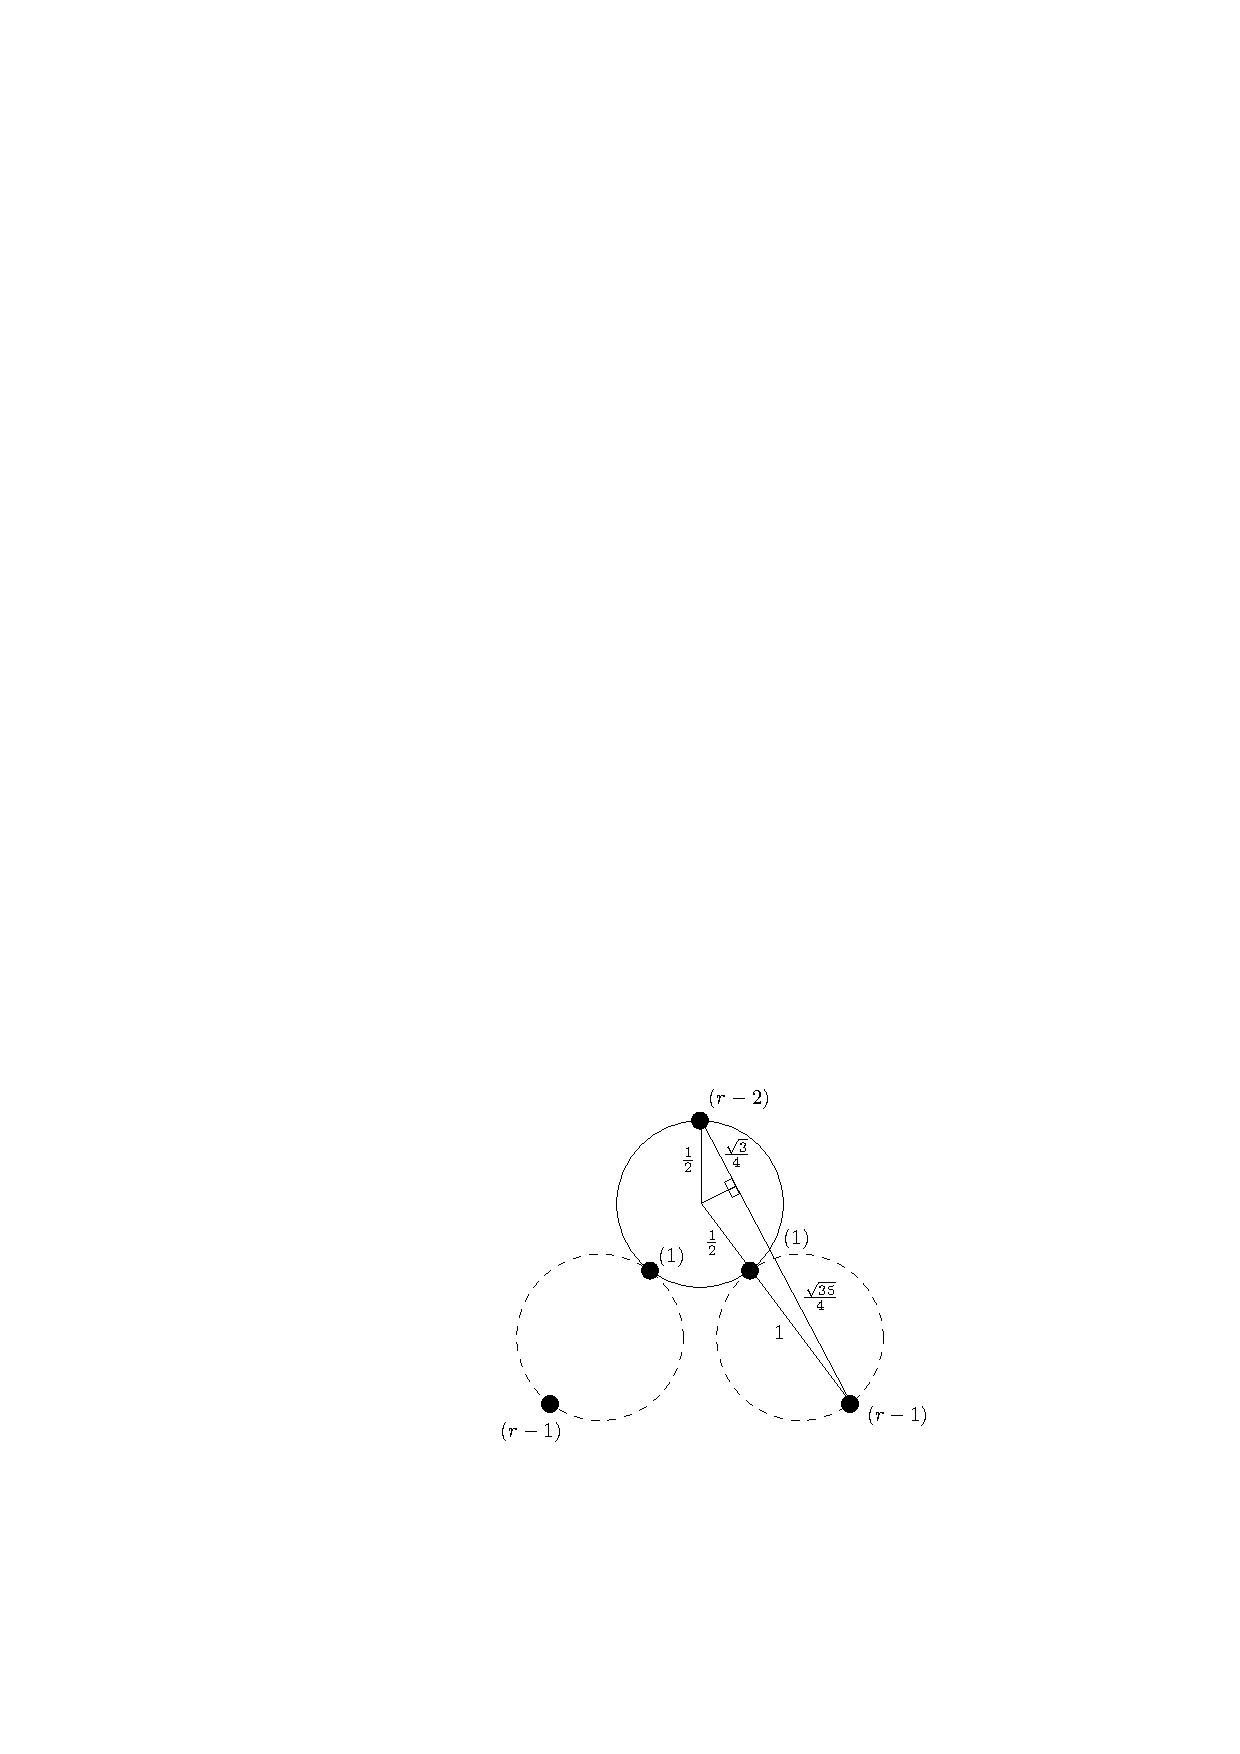
\includegraphics[scale=.9]{figs/splitter}
\caption{Splitter gadget}
\label{fig:splitter}
\end{center}
\vspace{-5pt}
\end{figure}

\begin{corollary}\label{cor:hardness5}
The $r$-gather problem in the $L_1$ and $L_\infty$ metrics is NP-hard to approximate better than a factor of 2.
\end{corollary}

\begin{theorem}\label{thm:hardness3}
The $r$-gather problem for the case where the diameter of a cluster is the distance between the furthest pair of points, then it is NP-hard to approximate better than $\sqrt{2+\sqrt{3}} \approx 1.931$ when $r=3$ or $4$.
\end{theorem}

\begin{theorem}\label{thm:hardness4}
The $r$-gather problem for the case where the diameter of a cluster is measured by the diameter of the smallest covering disk is NP-hard to approximate better than a factor of $\sqrt{13}/2 \approx 1.802$ when $r=3$.
\end{theorem}

Corollary \ref{cor:hardness5} is consequence of Theorem \ref{thm:hardness1}.  Theorems \ref{thm:hardness3} and \ref{thm:hardness4} are proved with reductions from planar circuit SAT.  The gadgets used in the reduction are similar to the splitter gadget used in the proof of Theorem \ref{thm:hardness1}.  Details of the proofs are omitted due to space constraints.

%\begin{proof}
%We reduce from the NP-hard problem planar circuit SAT.  We are given a planar boolean circuit with a single output.  Similar to the previous proofs, a wire gadget consists of a line of points that alternate between a single point and a group of $r-1$ points at the same location.  The parity of the clusters chosen signify a true signal or a false signal.  When the clusters combine a group of $r-1$ points followed by a single point, the signal of the wire is true.  It is simple to enforce the output to be a true signal by ending the output wire with a single point.  The beginning of the input wires have a group of $r$ points so that the inputs can be either true or false.  Figure~\ref{fig:nandgadget} illustrates the NAND gadget, a universal gate.  The solid clusters illustrate two true inputs into the gate and a false output.  If either or both of the inputs is false, then two groups of points in the triangle (or all three) will become a cluster and the output will be true.  Figure~\ref{fig:splittercircuit} ilustrates the splitter circuit where the solid clusters indicate a true signal and the dashed clusters indicate a false signal.  As before, if the optimal solution to the $r$-gather construction can be found, then cluster diameter will be 1.  Otherwise, three groups will form a cluster, two from the triangle and one adjacent to the triangle.  The diameter of such a cluster is $\sqrt{13}/2 \approx 1.802$ when $r=3$.  Finally, note that in order to connect the wires, they must be able to turn somehow.   We can bend the wire such that no three groups of points can form a cluster that has diameter smaller than $\sqrt{13}/2$.  Thus concludes our proof.
%\end{proof}

%\begin{figure}[htbp]
%\begin{center}
%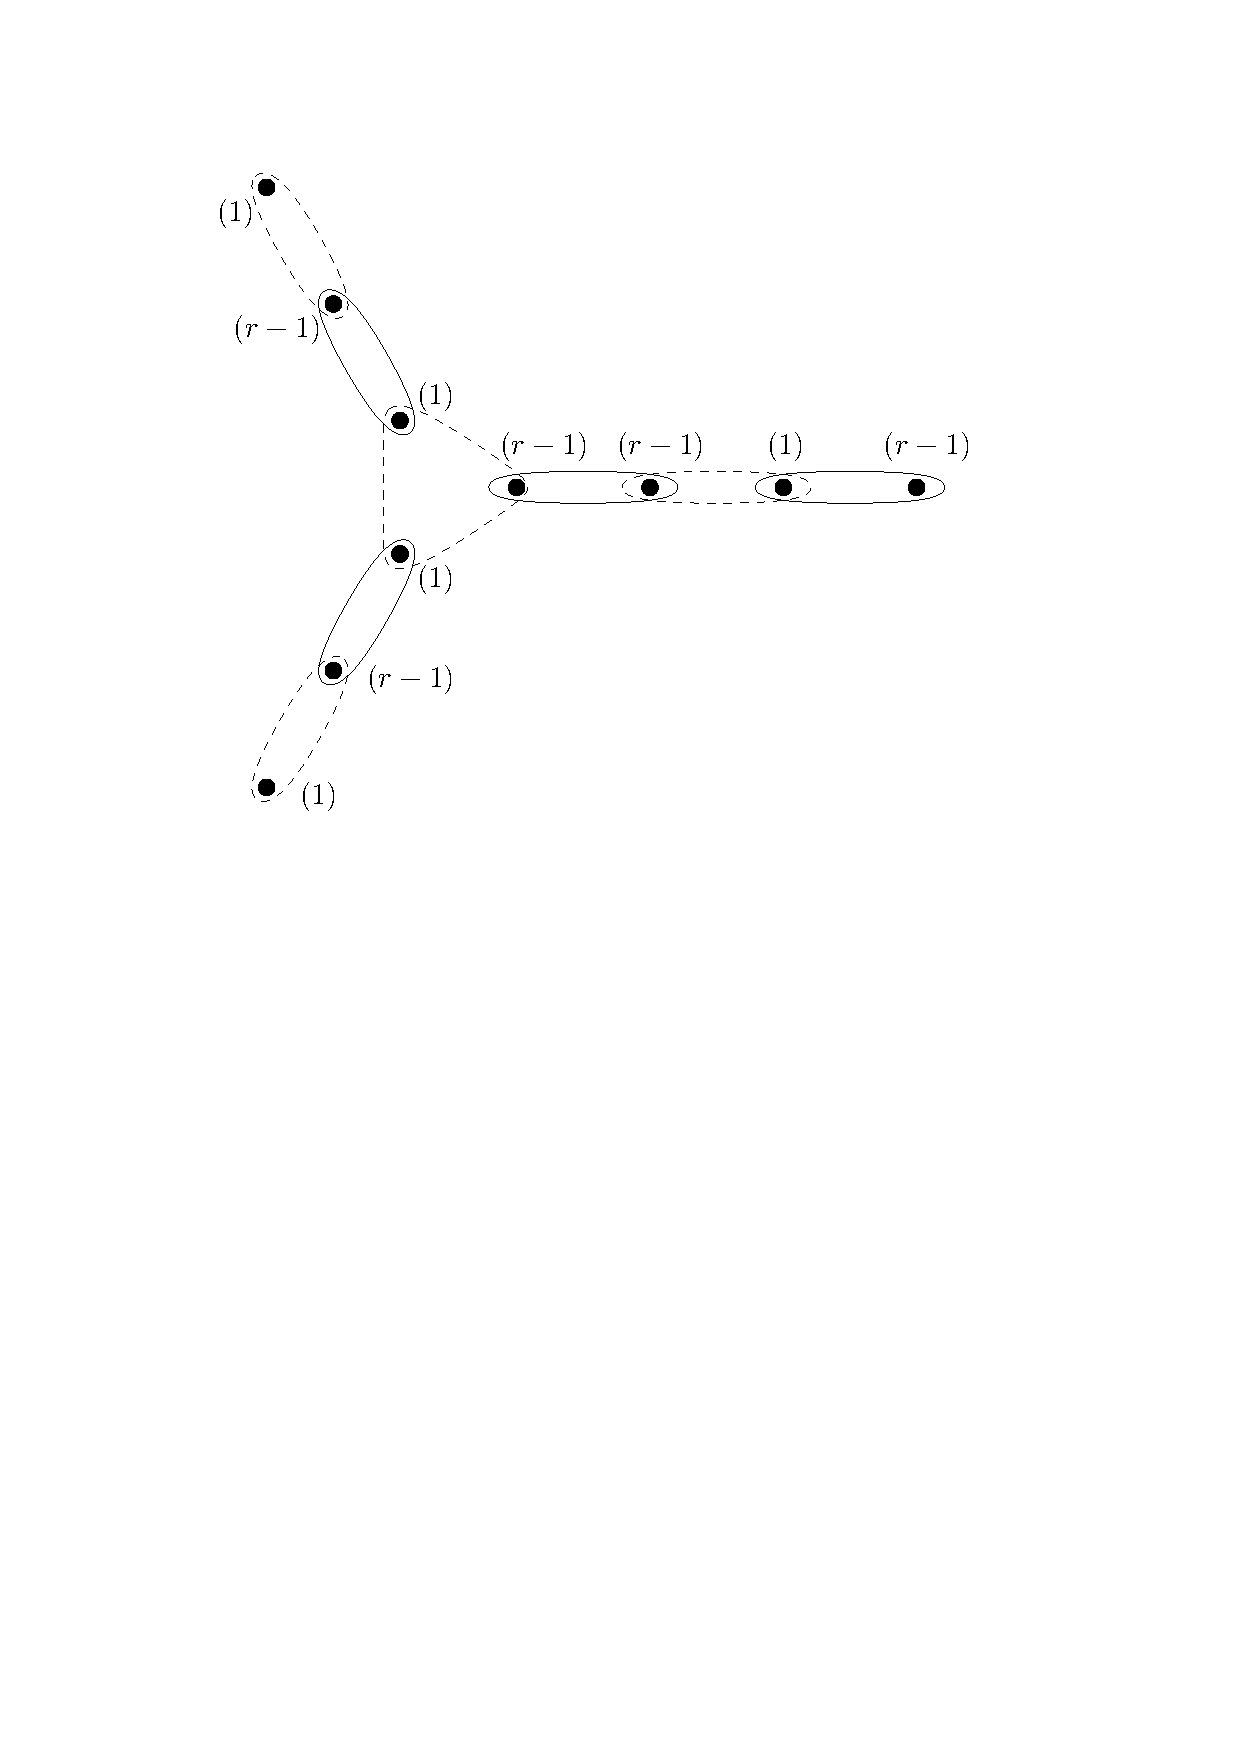
\includegraphics[scale=.6]{figs/nandgadget}
%\caption{NAND gadget}
%\label{fig:nandgadget}
%\end{center}
%\end{figure}

%\begin{figure}[htbp]
%\begin{center}
%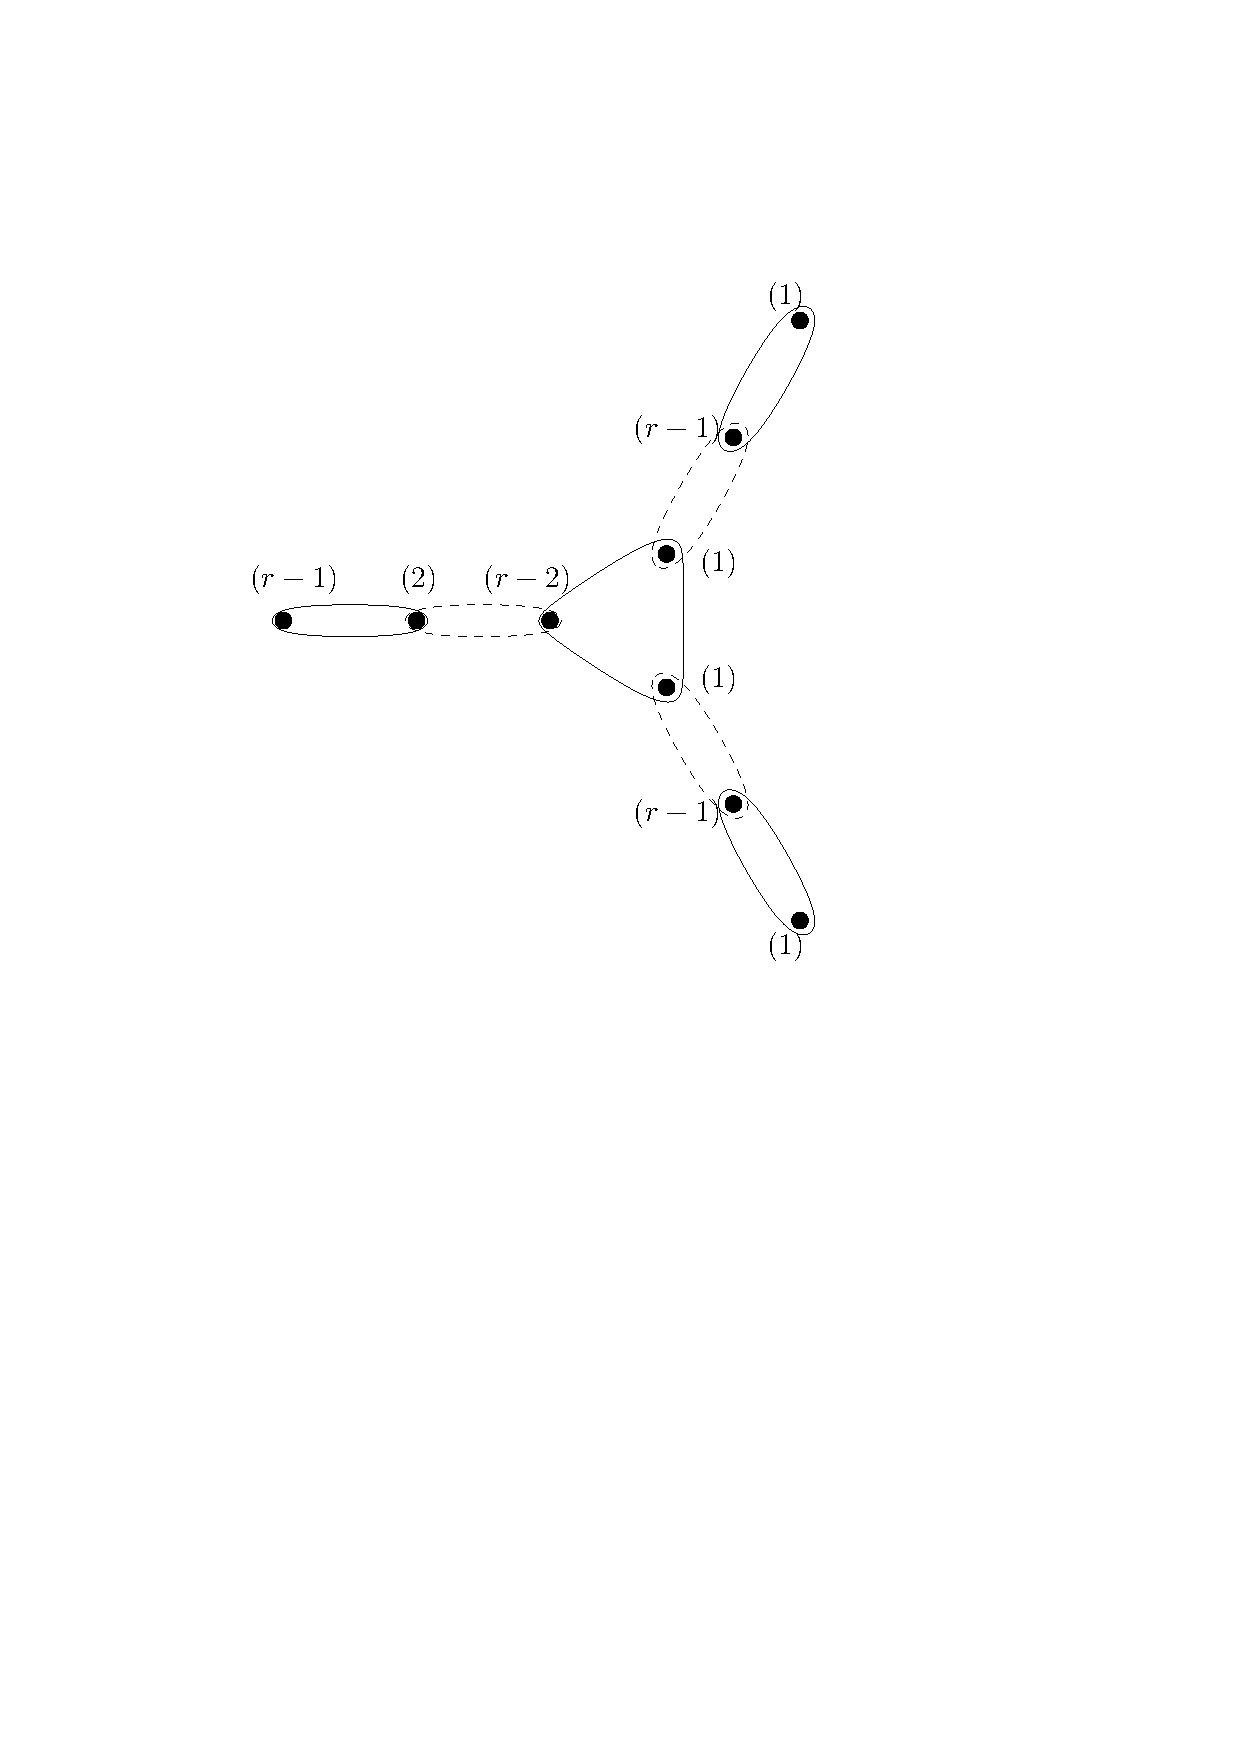
\includegraphics[scale=.6]{figs/splittergadget}
%\caption{splitter gadget}
%\label{fig:splittercircuit}
%\end{center}
%\end{figure}

\begin{small}
\bibliographystyle{abbrv}
\bibliography{r-gather}
\end{small}
\end{document}
